\chapter{Evaluation}\label{ch:evaluation}
% Using the previously presented implementation, you can now evaluate your approach.\\
% Get as many quantitative measurements as possible.  E.g. compare
% different implementations in terms of hardware usage, latency...\\
% This chapter is usually filled with graphs and numbers.  In the end, the
% numbers should show how your approach is better (in some regard) than
% existing approaches.
The objective of this evaluation is twofold: first, to verify that the design meets the
requirements set out in section \ref{system_requirements}, primarily throughput and packet
latency; and second, to assess the resource utilization of the design once synthesized, in
order to identify how efficiently it uses the available FPGA resources. Performance evaluation
is carried out through behavioral simulation of the  using the testbench described in
section \ref{sec:testbench-architecture}, while utilization is assessed separately through
out-of-context synthesis, as covered in \ref{sec:utilization}.

\section{Testbench architecture}\label{sec:testbench-architecture}

The design is evaluated using an almost UVM-like testbench shown in \ref{fig:tb}, built to allow controlled,
repeatable stimulus generation. It consists of three main components: a behavioral \gls{hbm} 
memory model, with independently configurable response latency and in-flight transaction depth for both read and write requests;
a UDP packet generator that drives the ingress side of the design and supports parametrizable packet length, number of flows,
interleaving between flows, and number of packets sent per flow; and finally, a simple \gls{fec} 
encoder model sitting on the egress side, which simply consumes whatever data the buffer forwards to it without
performing any encoding itself. \\

All three components (the packet generator, the \gls{hbm} model, and the encoder model) communicate with the design under test over the same
\gls{axi}-Stream interfaces described in chapter \ref{ch:implementation}. Besides the aforementioned components, 
both the packet generator and encoder model are connected to a global scoreboard that keeps track of all the sent packets, and eventually 
provides the latency and throughput metrics.

\begin{figure}
  \begin{center}
    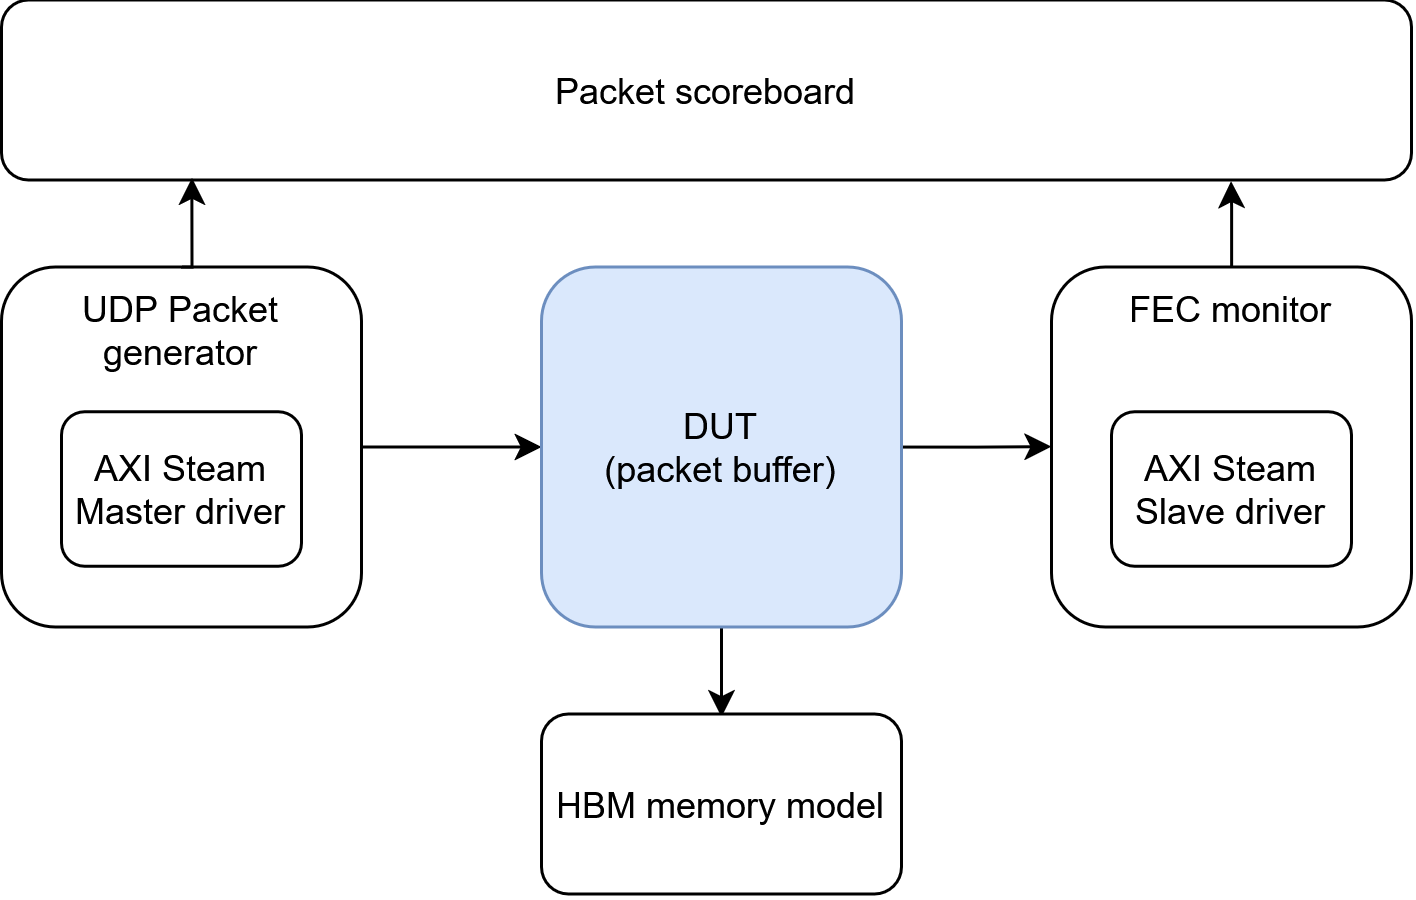
\includegraphics[width=0.95\textwidth]{../img/tb.png}
  \end{center}
  \caption{Testbench architecture}\label{fig:tb}
\end{figure}

\section{Waveform example}

Before turning to aggregate performance numbers, it is useful to look at a single, simple
run of the design to confirm that the datapath behaves as intended. Figure~\ref{fig:waves} shows a
simulation waveform for a minimal case in which four packets, all belonging to the same flow,
are fed into the buffer with the generation size configured to four. \\

The four packets are written in order and are eventually forwarded to the encoder together, once the full
generation is available. The waveform also shows the free memory queue and the flow's packet
descriptor queue being popped and pushed, respectively, as each packet is written: notably,
the free memory queue is popped right as the corresponding \gls{axi} write requests to \gls{hbm}
begin, i.e. the memory requests begin before the packet has fully arrived at the write engine, rather than only after the
whole packet has been buffered locally.

\begin{figure}
  \begin{center}
    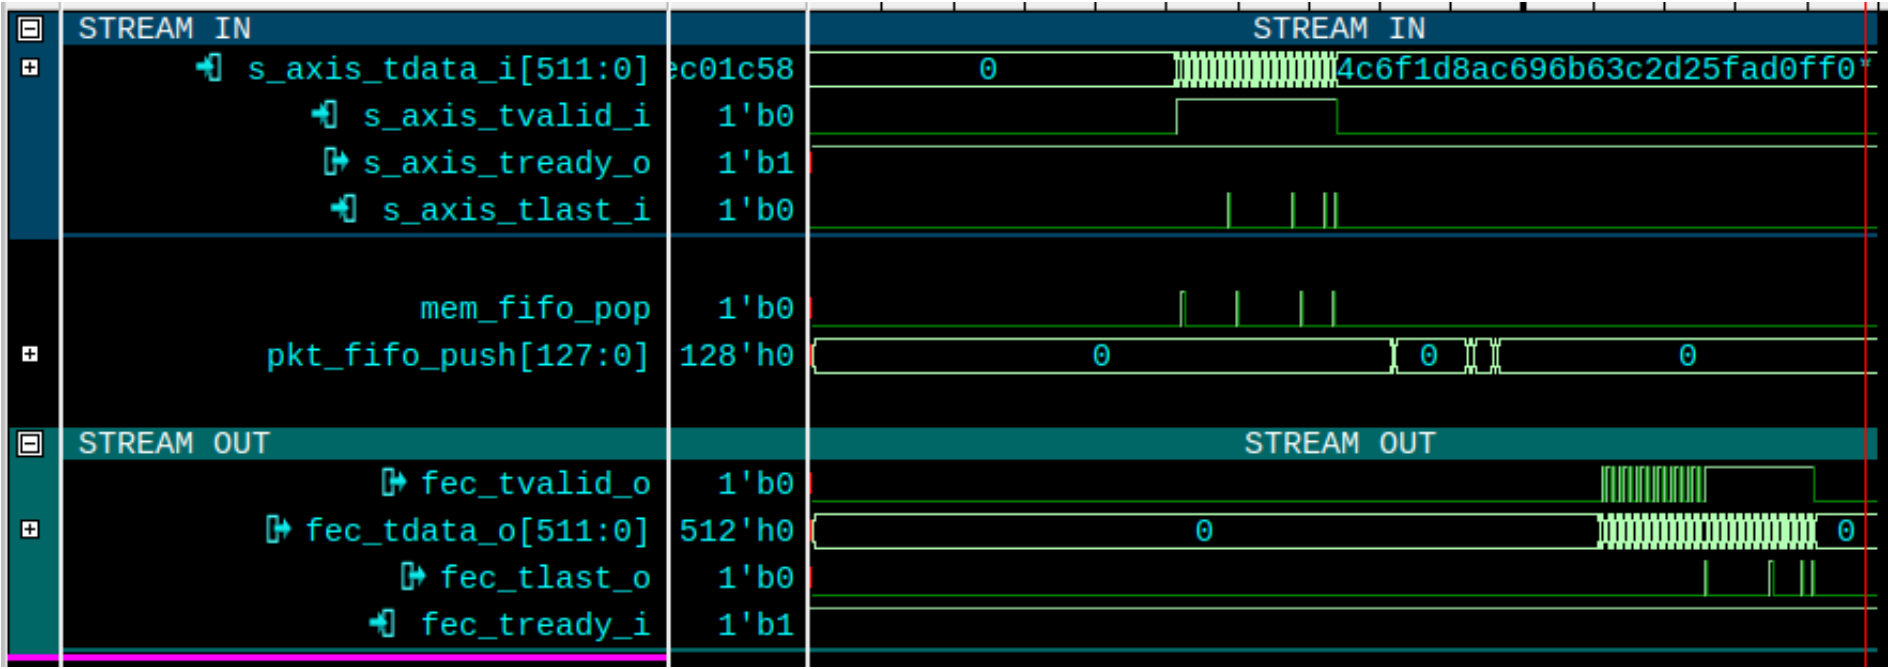
\includegraphics[width=0.95\textwidth]{../img/waves.png}
  \end{center}
  \caption{Simulation waveform}\label{fig:waves}
\end{figure}

\section{Performance evaluation}

Beyond confirming functional correctness, the design must also be shown to meet the
requirements set out in Section~\ref{system_requirements}, namely sustaining 100 Gb/s
of throughput and keeping packet latency low enough that the \gls{fec} encoder itself
dominates the end-to-end delay. The remainder of this chapter therefore evaluates the buffer
along these two axes. Unless explicitly stated otherwise, every measurement in this chapter
uses the example configuration introduced in Section~\ref{subsec:assumptions} (generation size 32,
128 flows, a free memory queue depth of 1024, and a per-flow queue depth of 64).

\subsection{Test suite and configs}

Three sweeps are used to characterize the design's behavior along different axes: the packet
size sweep evaluates raw throughput and latency as a function of packet size, the
interleaving sweep evaluates how the pattern in which packets from different flows
arrive affects latency, and the configuration sweep evaluates how scaling the
design's parameters (generation size, flow count, and queue depths) affects both
throughput and latency.

\subsection{Packet size sweep}

The goal of this sweep is to evaluate raw throughput across a range of packet sizes. For this
test, 64 packets per flow are sent across 16 flows, in bursts of 16 packets at randomly
interleaved flow order, under three packet size variations: maximum-size (1500 B) packets,
minimum-size (46 B) packets, and randomly sized packets drawn from a uniform distribution.
Figure \ref{fig:pkt_sweep} shows the results. Throughput does not vary significantly across the
three cases, which is the expected and desirable outcome: it confirms that the memory
pipeline, built around multiple outstanding in-flight \gls{hbm} requests, is working as
intended rather than stalling between requests of different sizes. Latency shows a small but
consistent increase for larger packets, which follows directly from the longer time needed to
transfer a larger packet into \gls{hbm}.

\begin{figure}
  \begin{center}
    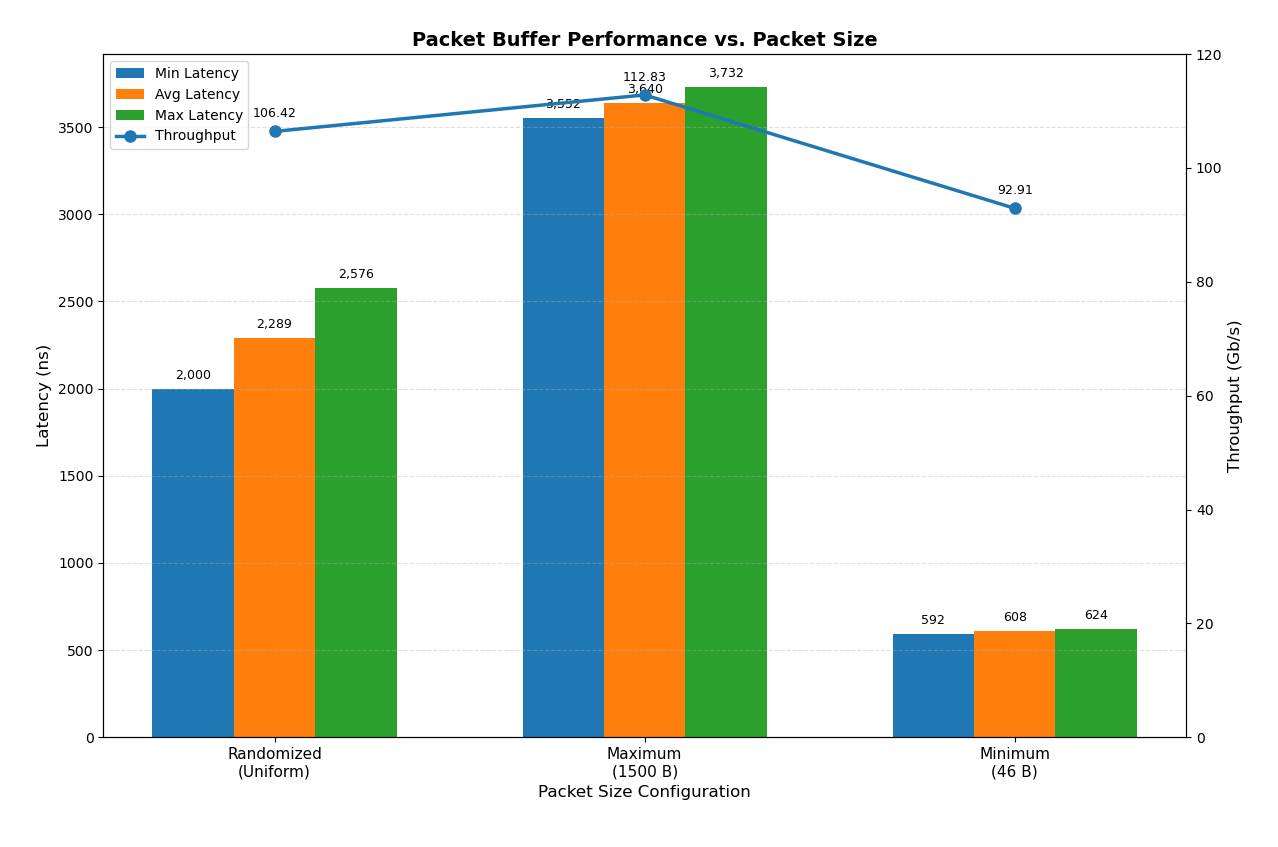
\includegraphics[width=0.95\textwidth]{../img/pkt_sweep_labeled.png}
  \end{center}
  \caption{Packet size sweep}\label{fig:pkt_sweep}
\end{figure}

\subsection{Interleaving sweep}

While the previous sweep focused on throughput, this sweep is aimed primarily at latency: it
evaluates how the order in which packets from different flows arrive affects the delay before
a generation becomes available to the encoder. For this test, 64 randomly sized packets per
flow are sent across 128 flows, under three interleaving patterns: a worst case, in which the
generator iterates over every flow sending one packet at a time (burst size of 1) before
returning to the first flow; a best case, in which the generator sends a full generation's
worth of packets (burst size of 32) to one flow before moving to the next; and a randomized
case, drawn from a uniform distribution over flows.\\

The worst-case pattern is also the easiest to reason about analytically, and is the only one
of the three for which a theoretical figure is given here, since it is dramatically larger
than the other two: for any given flow to complete a generation, the buffer must first receive
31 more packets from each of the other 127 flows, i.e. \(128 \times 31\) packets, before the
last packet of the reference flow's generation arrives. At the maximum packet size of 1500 B,
this amounts to 12.1 MB that must be transferred before the encoder receives anything, which at
100 Gb/s corresponds to a theoretical delay of approximately 970 $\mu$s. \\

The measured results, shown in figure \ref{fig:burst_sweep}, remain well below this theoretical
bound: the worst-case pattern yields an average latency of 116,415 ns and a
maximum latency of 349,623 ns, while the randomized pattern yields an average
latency of 37,616 ns and a maximum of 179,779 ns. That the
measured worst-case latency sits so far below the fully-serial theoretical estimate is
consistent with the memory pipeline's use of multiple outstanding in-flight requests, discussed
in Chapter~\ref{ch:implementation}: the 970 $\mu$s figure assumes every intervening
packet is transferred strictly one after another, whereas in practice several of these
transfers can be in flight simultaneously. \\

% The best-case scenario shows a mini
% \todo{Add the best-case (burst size 32) measured latency numbers here for completeness.}

\begin{figure}
  \begin{center}
    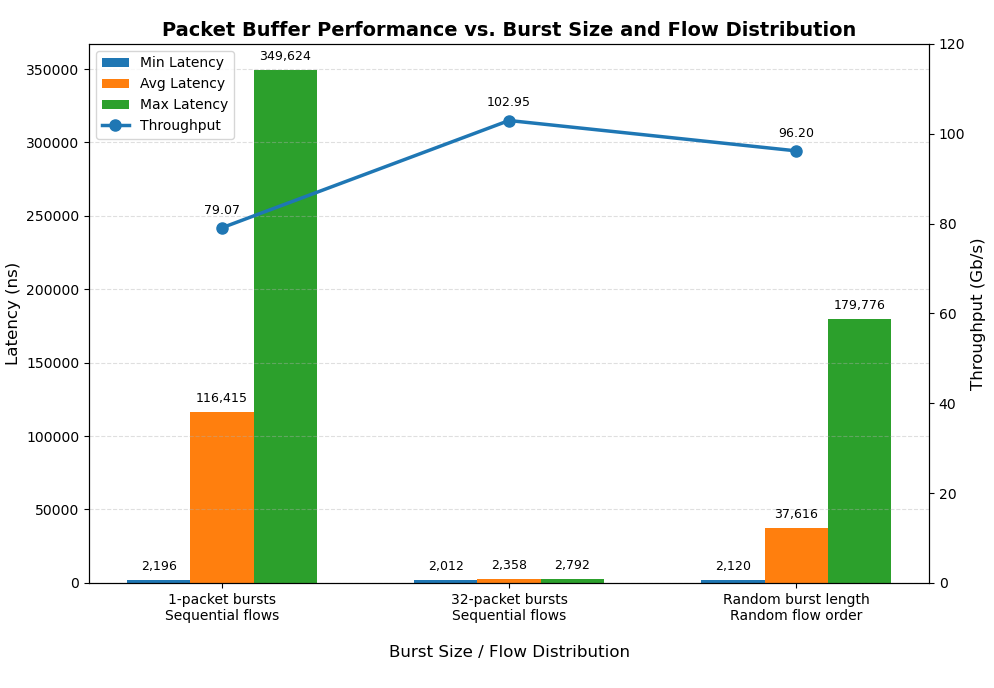
\includegraphics[width=0.95\textwidth]{../img/burst_sweep_labeled.png}
  \end{center}
  \caption{Burst size sweep}\label{fig:burst_sweep}
\end{figure}

\subsection{Configuration sweep}

This final sweep keeps the proportions between the design's parameters fixed, in particular,
the free memory queue and per-flow queue depths remain sized relative to the generation size
as in section \ref{subsec:assumptions}, while varying their absolute values, in order to see how
scaling the design up or down affects performance. As in the packet size sweep, 64 packets per
flow are sent across 16 flows. Figure~\ref{fig:cfg_sweep} shows that throughput remains roughly
similar across the swept configurations; the more significant effect is on packet latency,
where the generation size is the dominant factor, since a packet cannot be forwarded to the
encoder until its entire generation has been accumulated.

Table~\ref{tab:cfg-sweep} lists the three configurations tested. Each keeps the same ratios as the
example configuration of section \ref{subsec:assumptions}: the free memory queue depth is always 32
times the generation size, and the flow count is always 4 times the generation size.

\begin{table}[h]
  \centering
  \caption{Configurations tested in the configuration sweep}
  \label{tab:cfg-sweep}
  \begin{tabular}{lrrr}
    \hline
    & Generation size & Flows & Mem.\ queue depth \\
    \hline
    Baseline (example config) & 32 & 128 & 1024 \\
    Half-scale                & 16 & 64  & 512  \\
    Quarter-scale              & 8  & 32  & 256  \\
    \hline
  \end{tabular}
\end{table}

% \todo{Summarize the resulting throughput and latency numbers for each of the three configurations.}

\begin{figure}
  \begin{center}
    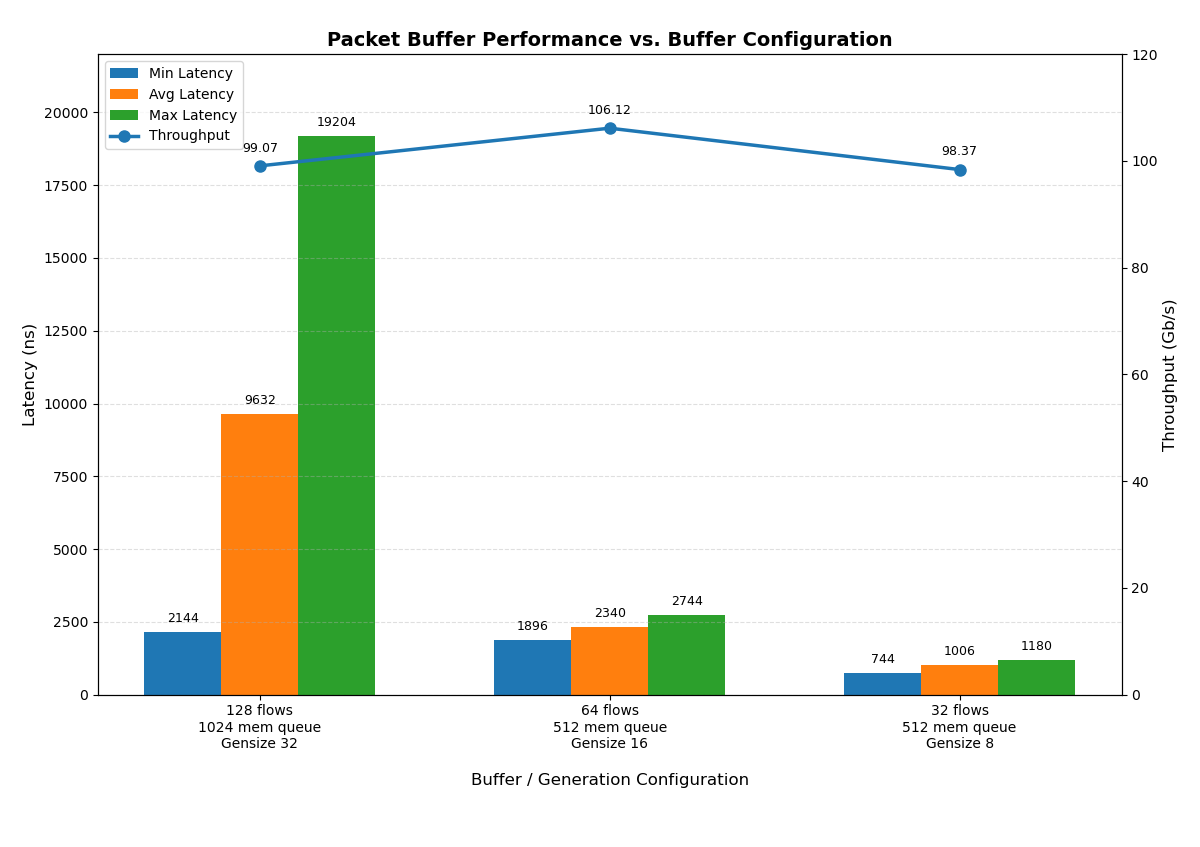
\includegraphics[width=0.95\textwidth]{../img/cfg_sweep_labeled.png}
  \end{center}
  \caption{Configuration sweep}\label{fig:cfg_sweep}
\end{figure}

\section{Utilization}\label{sec:utilization}

To obtain an early estimate of the design's resource cost independently of the surrounding
Open NIC Shell and HBM IP integration, an out-of-context synthesis of \texttt{packet\_buffer\_top} (the top top-level module in the hierarchy) 
was performed in Vivado using the example configuration of \cref{tab:example-config} 
(generation size 32, 128 flows, a free memory queue depth of 1024, and a per-flow queue depth 
of 64). \\

The diagram in \ref{fig:oob_util} shows the resulting utilization broken down by primitive type. As the
figure shows, the design is dominated by flip-flop usage: no block RAM (RAMB36/RAMB18), UltraRAM,
LUTRAM, or SRL resources are used anywhere in the hierarchy, meaning every queue and buffer in
the design is currently implemented purely as flop-based storage rather than being mapped onto
dedicated memory primitives. \\

\begin{figure}
  \begin{center}
    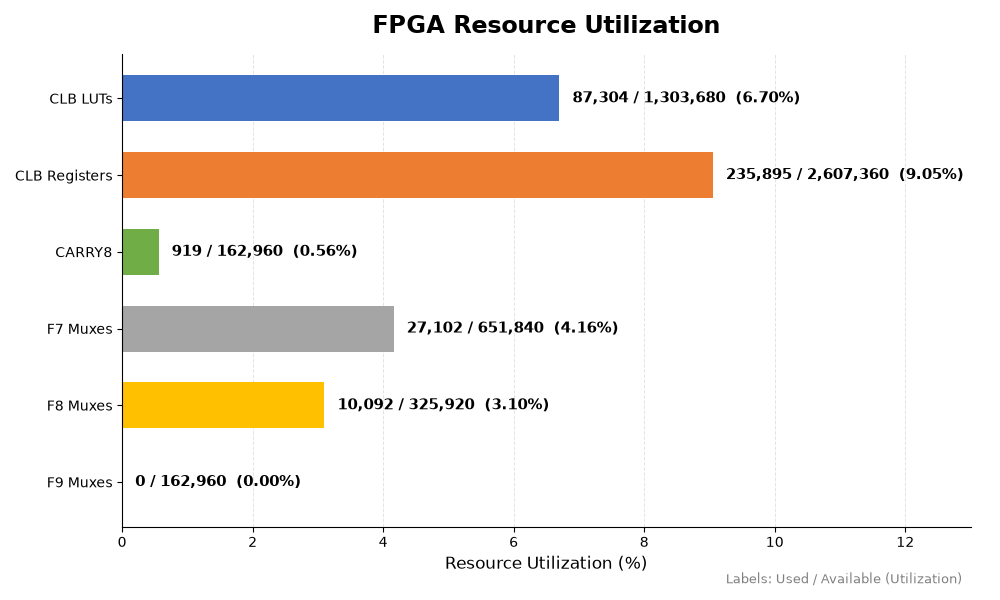
\includegraphics[width=0.95\textwidth]{../img/util.png}
  \end{center}
  \caption{FPGA utilization report}\label{fig:oob_util}
\end{figure}


Table \ref{tab:util-breakdown} decomposes the same synthesis run by pipeline stage, mapping each
top-level instance in the hierarchical utilization report back onto the stages introduced in
chapter \ref{ch:design}: flow ingest (\texttt{i\_flow\_ingest}), the packet writer
(\texttt{i\_pkt\_writer}, comprising both write-engine instances), the packet descriptor
queues (the 128 per-flow \texttt{fifo\_sync\_1r1w} instances under \texttt{gen\_pkt\_fifos}),
the free memory queue (\texttt{i\_mem\_fifo} together with the address-interleaving buffer
\texttt{pkt\_addr\_ilv\_buf}), and the packet reader (\texttt{i\_pkt\_reader}, comprising both
read-engine instances and the round-robin arbiter).


\begin{table}[h]
  \centering
  \begin{tabular}{lrrrr}
    \hline
    Stage & LUTs & \% of total & FFs & \% of total \\
    \hline
    Flow ingest                & 7{,}464  & 8.6\%  & 15{,}317  & 6.5\%  \\
    Packet writer              & 7{,}133  & 8.2\%  & 20{,}922  & 8.9\%  \\
    Packet descriptor queues   & 53{,}106 & 60.8\% & 150{,}130 & 63.6\% \\
    Free memory queue          & 5{,}030  & 5.8\%  & 13{,}554  & 5.7\%  \\
    Packet reader              & 14{,}571 & 16.7\% & 35{,}971  & 15.3\% \\
    \hline
    \textbf{Total}             & \textbf{87{,}304} & \textbf{100\%} & \textbf{235{,}895} & \textbf{100\%} \\
    \hline
  \end{tabular}
  \caption{Post-synthesis resource usage by pipeline stage (out-of-context, example configuration)} \label{tab:util-breakdown}
\end{table}

The packet descriptor queues alone account for roughly 61\% of the design's LUTs and 64\% of
its flip-flops, which is expected given that this stage instantiates one dedicated queue per
supported flow (128 in this configuration). More broadly, if every flop-based FIFO instance in
the design is counted (not only the per-flow packet descriptor queues, but also the smaller
FIFOs internal to the write and read engines (burst-instruction, chunking, pending-transaction,
and reassembly FIFOs) and the free memory queue itself) these FIFO primitives together account
for approximately 220{,}000 flip-flops, or over 90\% of the design's total register count. \\ 

In other words, the large majority of the design's flip-flop usage is not spent on control logic
at all, but on the flop-based FIFOs used throughout the datapath to hold queue and buffer state;
this is a direct consequence of the lack of block RAM or UltraRAM inference noted above, and is
addressed as a resource-optimization opportunity in chapter \ref{ch:implementation}.


